\chapter{Realisierung}
\label{cha:Realisierung}
Dieses Kapitel befasst sich mit der Implementierung der Spezifikation des Vorlagenmanagements, die in Kapitel \ref{cha:Lösungskonzept} vorgestellt wurde. Die Implementierung wurde in Java 8 mit dem \emph{Buildtool Maven} realisiert, wobei die Implementierungen in der Projektstruktur organisiert wurden, die in Abbildung \ref{fig:minimal-example:frame-dirtree} dargestellt ist.
\begin{figure}[h]
\dirtree{%
.1 mailing.
.2 model.
.3 jpa.
.2 module.
.3 template.
.4 cdi.
.4 jsf.
.4 model.
.5 json.
.4 logic.
.5 api.
.5 impl.
.3 integration.
.4 clevercure-web.
.2 testsuite.
.3 cdi.
.2 demo.
.3 logic.
.3 web.
.2 data.
.3 api.
.3 impl.
}
\caption{Die Verzeichnisstruktur der \emph{Maven}-Projekte}
\label{fig:minimal-example:frame-dirtree}
\end{figure}
\ \newline
Das \emph{Maven}-Wurzelprojekt \emph{mailing} organisiert alle benötigten Abhängigkeiten, sowie die auf alle Unterprojekte anwendbare \emph{Build}-Konfigurationen. Die übergeordneten Projekte sind vom Typ \emph{pom}, was bedeutet, dass aus diesen Projekten keine Artefakte erstellt werden können und die übergeordneten Projekte die tiefer liegenden Projekte bündeln. Die gesamte Organisation der Abhängigkeiten findet im Wurzelprojekt \emph{mailing} statt. Diese Projektstruktur wurde gewählt, da in diesem Projekt auch die Implementierungen der anderen Softwarekomponenten von \emph{CleverMail} organisiert werden. 
\newline
\newline
Die konkreten Artefakte wurden jeweils in ein Artefakt \emph{*-api} und \emph{*-impl} aufgeteilt, somit sind die Schnittstellen  vollständig getrennt von deren Implementierungen. 
\newline
\newline
Folgende Auflistung beschreibt alle konkreten Artefakte (\emph{Java-Archive}), die aus dem Wurzelprojekt \emph{mailing} erstellt werden können.
\begin{itemize}
	\item\emph{\textbf{mailing-model-jpa}} enthält die Klassen mit den \emph{JPA}-Entitäten, welche die Datenbank in \emph{Java} abbilden.
	\item\emph{\textbf{mailing-module-template-cdi}} enthält die Implementierung der \emph{CDI}-Erweiterung für die Integration in eine \emph{CDI}-Umgebung.
	\item\emph{\textbf{mailing-module-template-jsf}} enthält die Implementierung für die Integration in \emph{JSF}.
	\item\emph{\textbf{mailing-module-template-model-json}} enthält die Implementierung der \emph{JSON}-Datenobjekte in Form von \emph{Java}-Klassen.	
	\item\emph{\textbf{mailing-module-template-logic-api}} enthält die Spezifikation des Vorlagenmanagements.
	\item\emph{\textbf{mailing-module-template-logic-impl}} enthält die Implementierung der Spezifikation des Vorlagenmanagements.
	\item\emph{\textbf{mailing-module-integartion-clevercure-web}} enthält die Implementierung der Integration für die Anwendung \emph{CleverWeb}.
	\item\emph{\textbf{mailing-testsuite-cdi}} enthält die Ressourcen aller Tests, die in einer \emph{CDI}-Umgebung lauffähig sein müssen.
	\item\emph{\textbf{mailing-demo-logic}} enthält die Implementierung der Geschäftslogik der Beispielanwendung.
	\item\emph{\textbf{mailing-demo-web}} enthält die Webanwendung der Beispielanwendung.
	\item\emph{\textbf{mailing-data-api}} enthält die Spezifikation der Geschäftslogik, die die Persistenz der \emph{E-Mail}-Vorlagen behandeln. Es enthält auch die Datenbankzugriffsklassen in Form von \emph{Data-Repository}-Schnittstellen.
	\item\emph{\textbf{mailing-data-impl}} enthält die Implementierung der Spezifikation der Geschäftslogik.
\end{itemize} 

\section{Implementierung der Spezifikation}
Dieser Abschnitt behandelt die Implementierung der Spezifikation, die in Kapitel \ref{cha:Lösungskonzept} vorgestellt wurde. 

\subsection{Implementierungen für \emph{CKEditor}}
Wie im Abschnitt \ref{sec:sub-typescript-javascript} vorgegeben, wurde ein \emph{Plugin} in \emph{TypeScript} implementiert, das innerhalb des \emph{CKEditors} die Variablen verwaltet. Die Implementierung des \emph{Plugins} in \emph{TypeScript} war möglich, da für den \emph{Editor CKEditor} von dem \emph{Microsoft} verwalteten \emph{Open-Source}-Projekt \emph{DefinitelyTyped} Typinformationen für \emph{TypeScript} bereitgestellt werden, welche die \emph{JavaScript}-Schnittstellen als \emph{TypeScript}-Schnittstellen definieren. Wären keine Typinformationen zur Verfügung gestanden, hätte man die Typinformationen selber implementieren müssen, was einen erheblichen Mehraufwand bedeutet hätte.
 
\subsubsection{\emph{CKEditor-Plugin} in \emph{TypeScript}}
Das Variablenmanagement ist unabhängig vom verwendeten \emph{Editor} und wurde daher vom \emph{CKEditor-Plugin} logisch und physisch getrennt, wobei das Variablenmanagement im \emph{TypeScript}-Modul \emph{cc.variables} und das \emph{CKEDitor-Plugin} im \emph{TypeScript}-Modul \emph{cc.ckeditor.plugins} implementiert wurden. 
\newline
\newline
Die voneinander getrennten \emph{TypeScript}-Quelltextdateien werden beim Kompilieren in eine einzige \emph{JavaScript}-Quelltextdatei zusammengeführt. Mit der Organisation in eigenen \emph{TypeScript}-Modulen wird sichergestellt, dass nur explizit nach außen sichtbar gemachte (\emph{export MyType \{...\}}) Funktionen oder Typen außerhalb des Moduls referenziert werden können. Ein \emph{TypeScript}-Modul wird in ein korrespondierendes \emph{JavaScript}-Modul übersetzt. Die Verwendung von Modulen bringt auch den Vorteil, dass am \emph{Window}-Objekt nur das Objekt der Wurzel des Namensraums \emph{cc} gebunden ist, wodurch das \emph{Window}-Objekt nicht mit den eigenen \emph{JavaScript}-Objekten "verschmutzt" wird. Die Quelltexte \ref{prog:example-typescript-modul} und \ref{prog:example-javascript-modul} zeigen ein \emph{TypeScipt}-Modul und das daraus resultierende \emph{JavaScript}-Modul.
\newpage

\begin{program}[h]
\caption{Das \emph{TypeScript}-Modul}
\label{prog:example-typescript-modul}
\begin{JsCode}[numbers=none]
module cc.ckeditor.plugins {
	export module variables {
		export interface VariableMapping {
	        id:string
		}
	}
}                  
\end{JsCode}
\end{program}

\begin{program}[h]
\caption{Das \emph{JavaScript}-Modul}
\label{prog:example-javascript-modul}
\begin{JsCode}[numbers=none]
var cc;
(function (cc) {
    var variables;
    (function (variables_1) {
    // The interface VariableMapping is not part of the generated JavaScript
    })(variables = cc.variables || (cc.variables = {}));
})(cc || (cc = {}));                 
\end{JsCode}
\end{program}
\ \newline
Die \emph{TypeScript}-Schnittstelle \emph{VariableMapping} aus dem Quelltext \ref{prog:example-typescript-modul} ist nicht Teil des generierten \emph{JavaScript}-Moduls, da diese Schnittstelle nur eine Typinformation für \emph{TypeScript} darstellt. Wäre die Schnittstelle \emph{VariableMapping} eine \emph{TypeScript}-Klasse, dann wäre diese Klasse auch Teil des generierten \emph{JavaScript}-Moduls und würde als \emph{JavaScript}-Funktion abgebildet werden.
\newline
\newline
[\cite{typeScriptDoc}] beschreibt einleitend die  \emph{TypeScript}-Schnittstellen in der Dokumentation von \emph{TypeScript} wie folgt.
\begin{quote}
	\emph{One of TypeScript’s core principles is that type-checking focuses on the shape that values have. This is sometimes called “duck typing” or “structural subtyping”. In TypeScript, interfaces fill the role of naming these types, and are a powerful way of defining contracts within your code as well as contracts with code outside of your project.}
\end{quote}
Das Variablenmanagement in \emph{TypeScript} ist verantwortlich für die \emph{Browser}-seitige Registrierung der Variablen und stellt Hilfsmethoden zur Verfügung, mit denen Variablen in der \emph{HTML}-Vorlage gefunden und konvertiert werden können. Der Quelltext \ref{prog:example-typescript-convert-variable} zeigt mehrere Möglichkeiten, wie eine Variable in \emph{TypeScript} konvertiert werden kann.
\newpage

\begin{program}[h]
\caption{Die Variablenkonvertierung in \emph{TypeScript}}
\label{prog:example-typescript-convert-variable}
\begin{JsCode}
// Helper class for the variable conversion
class VariableUtils {

    private variables:VariableMapping[] = [];
	
    // public function for the variable conversion
    public convert(converter:(item:VariableMapping) => any 
    	                    = (item:VariableMapping)=> item):any[] {
        var converted:any[] = [];
        for (var i = 0; i < this.variables.length; i++) {
            converted[i] = converter(this.variables[i]);
        }
        return converted;	            
    } 
    
}

// Separate class for the variable conversion
class MyConverter {
    // public function for the variable conversion
    public convert(v:VariableMapping): any {
        return v.displayName;
    }    
}

// Create objects of the defined types
var util     :VariableUtils = new VariableUtils();
var converter:MyConverter   = new MyConverter();

// Conversion via an arrow function
util.convert((v:VariableMapping) => v.displayName);

// Conversion via an anonymous function
util.convert(function (v:VariableMapping) { return v.displayName; });

// Conversion via a referenced function
util.convert(converter.convert);
\end{JsCode} 
\end{program}
\ \newline
Die Funktion \emph{convert} der Klasse \emph{VariableUtils} aus dem Quelltext \ref{prog:example-typescript-convert-variable} definiert den Formalparameter \emph{converter} als eine \emph{Arrow}-Funktion, welche die Signatur der Funktion für die Konvertierung definiert und eine Standardimplementierung definiert, die verwendet wird, wenn bei der Aktivierung der Funktion \emph{convert} für den Formalparameter \emph{converter} kein Aktualparameter bereitgestellt wird. Eine \emph{Arrow}-Funktion ähnelt einem \emph{Lambda}-Ausdruck in Java. Der Typ \emph{any[]} ist vergleichbar mit dem Datentyp \emph{dynamic} aus C\# und gibt an, dass jeder Datentyp als Typ des zurückgelieferten \emph{Arrays} erlaubt ist.

\subsubsection{Variablenrepräsentation in \emph{TypeScript}}
Eine Variable wird \emph{Java}-seitig als Objekte des Datentyps \emph{VariableContract} abgebildet, und muss für das \emph{JavaScript}-seitige Variablenmanagement in eine \emph{JSON}-Zeichenkette überführt werden, die als \emph{JavaScript}-Objekt innerhalb von \emph{JavaScript} verwendet wird. Dafür wurde in \emph{TypeScript} die Schnittstelle \emph{VariableMapping} aus dem Quelltext \ref{prog:example-typescript-variable-mapping} definiert, welche den Kontrakt einer Variable innerhalb von \emph{TypeScript} definiert.
\begin{program}[h]
\caption{Die \emph{TypeScript}-Schnittstelle \emph{VariableMapping}}
\label{prog:example-typescript-variable-mapping}
\begin{JsCode}
interface VariableMapping {  
    id   :string,       
    label:string,        
    info :string
}
\end{JsCode}
\end{program}
\ \newline
Die Schnittstelle \emph{VariableMapping} ist Teil des Moduls \emph{cc.variables},  wird mit dem \emph{TypeScript}-Schlüsselwort \emph{export} nach außen offengelegt und kann über den vollständigen Pfad \emph{cc.variables.VariableMapping} innerhalb von \emph{TypeScript} referenziert werden. Mit der Schnittstelle \emph{VariableMapping} werden Typinformationen für die Variablenpräsentation in \emph{TypeScript} bereitgestellt, damit innerhalb von \emph{TypeScript} die Typsicherheit sichergestellt werden kann.

\subsubsection{Variablenrepräsentation in \emph{Java}}
Die Klasse \emph{VariableJson} aus dem Quelltext \ref{prog:variableJson} zeigt die korrespondierende \emph{Java}-Implementierung der Variablenrepräsentation. Mit der Klasse \emph{VariableJson} wird sichergestellt, das die Variablenrepräsentation in \emph{Java} korrespondierend zur Variablenrepräsentation in \emph{TypeScript} ist.
\newline
\newline
Die Klasse \emph{VariableJson} stellt die Schnittstelle der Variablen, die in \emph{Java} über die Schnittstelle \emph{VariableContract} abgebildet sind, zu \emph{TypeScript} bzw. \emph{JavaScript} dar. Als \emph{JSON-Provider} wird die Bibliothek \emph{FasterXML-Jackson-JSON} [\cite{fasterXml}], vormals \emph{Jackson-JSON} genannt, verwendet, die es erlaubt mit Annotationen deklarativ Attribute und/oder Methoden einer Klasse auf \emph{JSON}-Attribute abzubilden. Durch den deklarativen Ansatz über Annotationen sind die annotierten  Attribute und/oder die annotierten Methoden einer Klasse entkoppelt von der Repräsentation in \emph{JSON} und können daher abgeändert werden ohne die Abbildung auf \emph{JSON} zu beeinflussen. Nur ein Ändern des Datentyps eines Attributes oder des Rückgabewerts einer Methode wird zu Problemen führen. 
\newline
\begin{program}
\caption{Die Klasse \emph{VariableJson}}
\label{prog:variableJson}
\begin{JsCode}
@JsonTypeName(value = "variable-json")
public class VariableJson extends AbstractJsonModel {

    private String id;
    private String label;
    private String info;

    public VariableJson() {
    }
    
    public VariableJson(String id, String label, String info) {
        this.id    = id;
        this.label = label;
        this.info  = info;
    }

    @JsonGetter("id")
    public String getId() { 
       return id; 
    }

    @JsonSetter("id")
    public void setId(String id) { 
       this.id = id; 
    }

    @JsonGetter("label")
    public String getLabel() { 
       return label; 
    }

    @JsonSetter("label")
    public void setLabel(String label) { 
       this.label = label; 
    }

    @JsonGetter("info")
    public String getInfo() { 
       return info; 
    }

    @JsonSetter("info")
    public void setInfo(String info) { 
       this.info = info; 
    }
    
}
\end{JsCode}
\end{program}
\ \newline

\subsubsection{Registrierung des \emph{Plugins} im \emph{CKEditor}}
Das \emph{Plugin} wird über eine \emph{JavaScript}-Datei im \emph{CKEditor} registriert, wobei folgende Konventionen eingehalten werden müssen:
\begin{itemize}
	\item\emph{ckeditor/plugins} ist das Verzeichnis, in dem das \emph{Plugin} enthalten sein muss.
	\item\emph{variables} ist das Verzeichnis unterhalb des Verzeichnisses \emph{ckeditor/plugins}, in dem die \emph{Plugin}-Ressourcen enthalten sein müssen und das den gleichen Namen haben muss wie das \emph{Plugin}.
	\item\emph{plugin.js} ist die \emph{JavaScript}-Datei, die im Verzeichnis \emph{ckeditor/plugins/variables} liegen muss und das implementierte \emph{Plugin} ist. 
\end{itemize}
\ \newline
Der Quelltext \ref{prog:example-ckeditor-config-js} zeigt einen Auszug aus der \emph{JavaScript}-Datei, mit der das \emph{Plugin} registriert wird und auch Einstellungen am \emph{CKEditor} vorgenommen werden können. Das \emph{Plguin} wird vom \emph{CKEditor} nach der Initialisierung des \emph{Editors} geladen und registriert.

\begin{program}[h]
\caption{Die Konfigurationsdatei für den \emph{CKEditor}}
\label{prog:example-ckeditor-config-js}
\begin{JsCode}
CKEDITOR.editorConfig = function (config) {
    // Register plugin variables
    config.extraPlugins = "variables";
}
\end{JsCode} 
\end{program}

\subsubsection{Integration des \emph{Plugins} im \emph{CKEditor}}
Die Abbildung \ref{fig:ckeditor-toolbar-opne-dialog} zeigt die Funktionsleiste des \emph{CKEditors}, in die der rot markierte \emph{Button} über das \emph{Plugin} eingefügt wurde. Durch einen Klick auf diesen \emph{Button} wird ein Dialog geöffnet, über den die zur Verfügung stehenden Variablen ausgewählt werden können.
\begin{figure}[h]
\centering
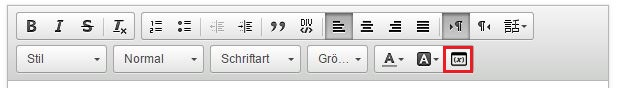
\includegraphics[scale=0.8]{ckeditor-toolbar-open-dialog}
\caption{Die \emph{CKEditor}-Funktionsleiste}
\label{fig:ckeditor-toolbar-opne-dialog}
\end{figure}
\ \newline
Die Abbildung \ref{fig:ckeditor-dialog-insert-variable} zeigt den Dialog, der vom \emph{CKEditor-Plugin} erstellt wurde. Im Dialog stehen alle registrierten Variablen zur Auswahl. Die Bezeichnung der ausgewählten Variable ist der Text in der Auswahlkomponente und die Beschreibung ist der Text, der unterhalb der Auswahlkomponente angezeigt wird. Durch einen Klick auf den \emph{Button OK} wird die Variable in die Vorlage eingefügt und der Dialog wird geschlossen.
\begin{figure}[h]
\centering
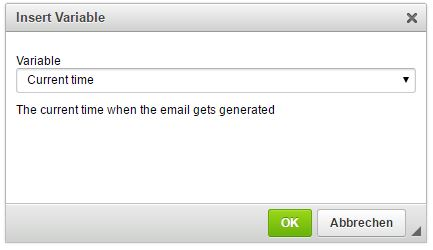
\includegraphics[scale=0.85]{ckeditor-dialog-insert-variable}
\caption{Der \emph{CKEditor} Dialog für die Variablenauswahl}
\label{fig:ckeditor-dialog-insert-variable}
\end{figure}
\ \newline
Die Abbildung \ref{fig:ckeditor-example-template} zeigt eine Vorlage innerhalb des \emph{CKEditors}, wobei die eingefügten Variablen hervorgehoben sind. Die Bezeichnung  der Variable stellt den Namen für den \emph{HTML-Tag} bereit und die Beschreibung dessen Titel. Die eingefügten \emph{HTML-Tags} dürfen nicht verändert werden, daher ist \emph{Drag}, \emph{Drop} und das Selektieren des eingefügten \emph{HTML-Tags} nicht erlaubt, da dadurch der eingefügte \emph{HTML-Tag} zerstört werden könnte und die Variablen nicht mehr gefunden werden können.
\begin{figure}[h]
\centering
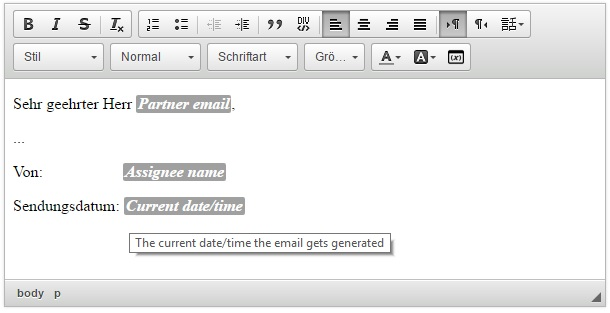
\includegraphics[scale=0.9]{ckeditor-example-template}
\caption{Beispiel einer Vorlage im \emph{CKEditor}}
\label{fig:ckeditor-example-template}
\end{figure}

\subsection{Implementierungen für \emph{CDI}}
\label{sec:sub-impl-integartion-cdi}
Dieser Abschnitt behandelt die Implementierung für die Integration in eine \emph{CDI}-Umgebung, wie in Abschnitt \ref{sec:sub-template-management-cdi} beschrieben. Die Variablen und Typen der Schnittstelle \emph{VariableResolverFactory} werden über eine \emph{CDI}-Erweiterung gefunden,  registriert und es werden die folgenden Ressourcen kontextabhängig über einen implementierten \emph{CDI}-Erzeuger zur Verfügung gestellt: 
\begin{itemize}
 \item Das Objekt des Datentyps \emph{VariableConfiguration} verwaltet die registrierten Variablen.
 \item Die Objekte des Datentyps \emph{TemplateDataJsonBuilder} erstellen das \emph{JSON}-Datenobjekt für eine Vorlage und eine spezifische \emph{Template-Engine}.
 \item Die Objekte des Datentyps \emph{TemplateProcessor} verwalten die Variablen in den Vorlagen.
 \item Objekte des Datentyps \emph{AbstractTemplateMetadata} halten die Metadaten der Vorlagen und werden spezifisch für eine \emph{Template-Engine} erstellt.
 \item Das Objekt der Klasse \emph{CdiTemplateUtil} konvertiert die registrierten Variablen, die Objekte des Datentyps \emph{VariableContract} sind, in Objekte der Klasse \emph{VariableJson}, wobei die Bezeichnung und die Beschreibung sprachspezifisch ermittelt werden.
\end{itemize}

\subsubsection{Vorlagenmanagement \emph{CDI}-Erweiterung}
Die implementierte \emph{CDI}-Erweiterung \emph{TemplateCdiExtension} hält die auffindbaren Ressourcen über die Lebensdauer der \emph{CDI}-Umgebung persistent. Eine \emph{CDI}-Erweiterung muss folgende Voraussetzungen erfüllen, um geladen und verwendet werden zu können:
\begin{enumerate}
	\item Sie muss die Schnittstelle \emph{javax.enterprise.inject.spi.Extension} implementieren,
	\item in einer Datei namens \emph{javax.enterprise.inject.spi.Extension}, die im Verzeichnis \emph{META-INF/services} liegen muss, mit ihrem voll qualifizierten Namen registriert werden und
	\item das Artefakt, dass die \emph{CDI}-Erweiterung enthält, muss eine Datei namens \emph{beans.xml} im Verzeichnis \emph{META-INF} enthalten.
\end{enumerate}
\ \newline
Die \emph{CDI}-Erweiterung wird beim Start der \emph{CDI}-Umgebung über den Mechanismus \emph{Service Provider Interface} (\emph{SPI}) geladen und ein Objekt der Klasse der \emph{CDI}-Erweiterung erstellt. Dann kann das Objekt der \emph{CDI}-Erweiterung auf Ereignisse des Lebenszyklus der \emph{CDI}-Umgebung reagieren, in dem die \emph{CDI}-Erweiterung Beobachtermethoden für die einzelnen Ereignisse implementiert, wie z.B.:
\begin{itemize}
	\item\emph{BeforeBeanDiscovery} ist das Ereignis, das einmalig beim Start der \emph{CDI}-Umgebung ausgelöst wird, bevor Typen, \emph{Beans} oder Injektionspunkte gesucht werden,
	\item\emph{ProcessAnnotatedType} ist das Ereignis, das für jeden gefundenen injizierbaren Typ ausgelöst wird und
	\item\emph{AfterBeanDiscovery} ist das Ereignis, das einmalig ausgelöst wird, wenn alle Typen, \emph{Beans} und Injektionspunkte gefunden und behandelt wurden.
\end{itemize}
\ \newline
Das erstellte Objekt der \emph{CDI}-Erweiterung ist an sich kein \emph{CDI-Bean}, da das Objekt der \emph{CDI}-Erweiterung bereits existiert, bevor die \emph{CDI}-Umgebung vollständig gestartet wurde, ist aber trotzdem in andere \emph{CDI-Beans} injizierbar. Alle anderen \emph{CDI-Beans} können erst nach dem erfolgreichen Start der \emph{CDI}-Erweiterung injiziert werden.
\newline
\newline
Der Quelltext \ref{prog:templateCdiExtension} zeigt einen Auszug aus der implementierten Klasse \emph{TemplateCdiExtension} und zeigt die Beobachtermethoden, die auf Lebenszyklusereignisse der \emph{CDI}-Umgebung reagieren. Die  \emph{CDI}-Erweiterung \emph{TemplateCdiExtension} findet
\begin{itemize}
	\item alle implementierten Typen der Schnittstelle \emph{VariableContract}, die mit der Annotation \emph{CdiVariableContract} annotiert sind und
	\item alle implementierten Typen der Schnittstelle \emph{VariableResolverFactory}, die mit der Annotation \emph{CdiVariableResolverFactory} annotiert sind.
\end{itemize}
\ \newline
Die gefunden Typen werden in der \emph{CDI}-Erweiterung registriert und über die Lebensdauer der \emph{CDI}-Umgebung verwaltet. Bezüglich der Typen der Schnittstelle \emph{VariableContract} sei angemerkt, dass zur Zeit nur implementierte Aufzählungstypen gefunden werden können. Alle Typen der Schnittstelle \emph{VariableContract}, die nicht ein Aufzählungstyp sind verursachen einen Fehler und verhindern einen Start der \emph{CDI}-Umgebung. Die Variablen könnten auch über implementierte Klassen der Schnittstelle \emph{VariableContract} definiert werden und bei ihrer Verwendung dynamisch aus der \emph{CDI}-Umgebung geholt werden, was zur Zeit nicht benötigt wird.
\newline
\newline
Eine \emph{CDI}-Erweiterung ist eine injizierbare Ressource, die in jedes \emph{CDI-Bean} injiziert werden könnte, obwohl nur das Variablenmanagement sich das Objekt der \emph{CDI}-Erweiterung injizieren sollte. Es kann nicht verhindert werden, dass sich andere \emph{CDI-Beans} das Objekt der \emph{CDI}-Erweiterung injizieren lassen, da eine \emph{CDI}-Erweiterung öffentlich deklariert werden muss.
\newpage

\begin{program}
\caption{Auszug aus der \emph{CDI}-Erweiterung \emph{TemplateCdiExtension}}
\label{prog:templateCdiExtension}
\begin{JavaCode}
public class TemplateCdiExtension implements Extension {

    private TemplateConfiguration templateConfig;
    private Map<Class<? extends VariableContract>, 
                Class<VariableResolverFactory>>  
                      variableResolverFactoryMap;

    void beforeBeanDiscovery(@Observes BeforeBeanDiscovery bbd) { ... }

    <T> void processCdiVariableContracts(
              @Observes @WithAnnotations({BaseName.class, 
                                          CdiVariableContract.class})
              ProcessAnnotatedType<T> pat) { ... }

    <T> void processVariableResolverFactories(
         @Observes @WithAnnotations(CdiVariableResolverFactory.class)
         ProcessAnnotatedType<T> pat) { ... }
         
}
\end{JavaCode}
\end{program}
\ \newline
Mit der folgenden Auflistung werden die implementierten Beobachtermethoden und deren Funktionsweise erklärt:
\begin{itemize}
	\item\emph{beforeBeanDiscovery} ist die Beobachtermethode, die alle Objekte erstellt, welche die gefundenen Typen über die Lebensdauer der \emph{CDI}-Umgebung verwalten,
	\item\emph{processCdiVariableContracts} ist die Beobachtermethode, welche die gefundenen Typen der Schnittstelle \emph{VariableContract} behandelt und
	\item\emph{processVariableResolverFactories} ist die Beobachtermethode, welche die gefundenen Typen der Schnittstelle \emph{VariableResolverFactory} behandelt.
\end{itemize}

\subsubsection{Vorlagenmanagement \emph{CDI}-Erzeuger}
Der implementierte \emph{CDI}-Erzeuger \emph{TemplateResourceProducer} produziert die kontextabhängigen Ressourcen des Vorlagenmanagements. Die Klasse \emph{TemplateResourceProducer} ist die einzige Klasse, in die das Objekt der \emph{CDI}-Erweiterung \emph{TemplateCdiExtension} injiziert wird. 
\newline
\newline
Im Kapitel \ref{cha:Lösungskonzept} wurde vorgegeben, dass mehrere \emph{Template-Engines} unterstützt werden müssen, daher wurde die Annotation \emph{@FreemarkerTemplate} eingeführt, die einen Injektionspunkt für die \emph{Template-Engine Freemarker} qualifiziert. In einer \emph{CDI}-Umgebung wird ein Qualifizierer benötigt, wenn für eine Schnittstelle mehrere Implementierungen zur Verfügung stehen, da ansonsten nicht entschieden werden kann, welche Implementierung verwendet werden soll. Für den Fall, dass es mehrere Implementierungen für eine Schnittstelle und nicht qualifizierte Injektionspunkte für diese Schnittstelle gibt, wird die Ausnahme \emph{AmbiguousResolutionException} ausgelöst und die \emph{CDI}-Umgebung kann nicht gestartet werden. 
\newline
\newline
Es wurden jeweils eine Erzeugermethode für den Qualifizierer \emph{@Default} und den Qualifizierer \emph{@FreemarkerTemplate} implementiert, womit nicht qualifizierte sowie qualifizierte Injektionspunkte versorgt werden können. Für die Erzeugermethode für den Qualifizierer \emph{@Default} wird die Implementierung für den Qualifizierer \emph{@FreemarkerTemplate} verwendet, wodurch diese Implementierung als die Standardimplementierungen fungiert. Damit setzt man sich jedoch der Gefahr aus, dass die produzierte Standardimplementierung nicht die gewollte Implementierung ist, daher ist Vorsicht geboten, wenn dieses Verhalten geändert werden sollte. 
\newline
\newline
Der Quelltext \ref{prog:templateResourceProducer} ist ein Auszug aus der Klasse \emph{TemplateResourceProducer} und zeigt einige der implementierten Erzeugermethoden. 
\newline
\newline
Die beiden Methoden \emph{produceDefaultTemplateBuilder} und \emph{produceFreeMarkerTemplateBuilder} produzieren Objekte des Datentyps  \emph{TemplateDataJsonBuilder} für den sogenannten Pseudo-Geltungsbereich (\emph{@Dependent}), wobei für jeden Injektionspunkt ein neues Objekt erstellt wird. Der Lebenszyklus von \emph{CDI-Beans}, die sich im Pseudo-Geltungsbereich befinden, wird nicht von der \emph{CDI}-Umgebung verwaltet und die Lebensdauer eines \emph{CDI-Beans}, das sich im Pseudo-Geltungsbereich befindet, ist gebunden and das \emph{CDI-Bean}, das sich das \emph{CDI-Bean} im Pseudo-Geltungsbereich injiziert hat. Die Erzeugermethoden \emph{produceDefaultTemplateBuilder} und \emph{produceFreeMarkerTemplateBuilder} lassen sich als Argument ein Objekt des Datentyps  \emph{VariableResolverFactoryProvider} injizieren, dessen Geltungsbereich für diese Methoden nicht bekannt und auch irrelevant ist.
\newline
\newline
Die Methode \emph{produceConfiguration} produziert ein Objekt des Datentyps  \emph{VariableConfiguration}, das die registrierten Variablen enthält und von der \emph{CDI}-Erweiterung bereitgestellt wird. Nachdem die Schnittstelle  \emph{VariableConfiguration} nur lesenden Zugriff erlaubt, wird dieses Objekt für den Gültigkeitsbereich der Anwendung produziert, also einmalig für die gesamte Lebensdauer der \emph{CDI}-Umgebung.
\newline
\newline
Alle injizierbaren Objekte, die sich in einem normalen Geltungsbereich befinden,  werden erst beim ersten Zugriff auf eine ihrer öffentlichen Methoden erzeugt und im korrespondierenden Geltungsbereich registriert. Sollte ein injizierbares Objekt niemals verwendet werden, so wird es auch niemals erzeugt. Dieses Verhalten ist möglich, da alle Injektionspunkte von \emph{Proxies}, außer Injektionspunkte von \emph{CDI-Beans} im Pseudo-Geltungsbereich, verwaltet werden, die beim Erstellen eines \emph{CDI-Beans} in die Injektionspunkte injiziert werden und ein abgeleiteter Typ des injizierten Typs sind. Bei einem Zugriff auf eine öffentliche Methode des injizierten Objekts, wird das korrespondierende Objekt aus dem aktuellen Geltungsbereich geholt oder vorherig erstellt und im Geltungsbereich abgelegt und der Aufruf an dieses Objekt weiter delegiert. 

\begin{program}[h]
\caption{Die Klasse \emph{TemplateResourceProducer}}
\label{prog:templateResourceProducer}
\begin{JavaCode}
@ApplicationScoped
public class TemplateResourceProducer implements Serializable {

    @Produces
    @ApplicationScoped
    @Default
    public VariableConfiguration produceConfiguration() {
        return extension.getVariableConfiguration();
    }
    
    @Produces
    @Dependent
    @Default
    public TemplateDataJsonBuilder produceDefaultTemplateBuilder
          (final @Default VariableResolverFactoryProvider factory) {
        return produceFreeMarkerTemplateBuilder(factory);
    }

    @Produces
    @Dependent
    @FreemarkerTemplate
    public TemplateDataJsonBuilder produceFreeMarkerTemplateBuilder
           (final @Default VariableResolverFactoryProvider factory) {
        return new FreemarkerTemplateDataJsonBuilder()
                      .withWeakMode()
                      .withVariableResolverFactoryProvider(factory);
    }
    
}
\end{JavaCode}
\end{program} 

\subsubsection{Vorlagenmanagement \emph{CDI}-Hilfsklasse}
Die Klasse \emph{CdiTemplateUtil} aus dem Quelltext \ref{prog:cdiTemplateUtil} wurde implementiert, um ein injizierbares \emph{CDI-Bean} zur Verfügung zu stellen, das Hilfsmethoden für die Konvertierung der Variablen von Objekten des Datentyps \emph{VariableContract} in Objekte der Klasse \emph{VariableJson} und vice versa zur Verfügung stellt. Diese Implementierung hält keinen Status, daher kann dieses \emph{CDI-Bean} in den Geltungsbereich der Anwendung registriert werden. Die Verwendung des Objekts der Klasse \emph{CdiTemplateUtil} ist \emph{Thread-safe} weil
\begin{itemize}
	\item das Objekt keinen Status hält und
	\item das verwendete Objekt der Klasse \emph{TemplateConfiguration} nur lesenden Zugriff erlaubt.
\end{itemize}
\ \newline
Mit der Annotation \emph{@Typed} kann man einschränken, über welche Typen ein \emph{CDI-Bean} injizierbar ist, was hilfreich ist, wenn die Klasse eines \emph{CDI-Beans} mehrere Schnittstellen implementiert. Also bewirkt die Annotation \emph{@Typed(CdiTemplateUtil.class)}, dass dieses \emph{CDI-Bean} nur über den Typ \emph{CdiTemplateUtil} injizierbar ist. 

\begin{program}[h]
\caption{Die Klasse \emph{CdiTemplateUtil}}
\label{prog:cdiTemplateUtil}
\begin{JavaCode}
@ApplicationScoped
@Typed(CdiTemplateUtil.class)
public class CdiTemplateUtil implements Serializable {

    @Inject
    private VariableConfiguration config;

    public List<VariableJson> convertContractToJsonModel(
                                     final Locale locale) { ... }

    public List<VariableJson> convertContractToJsonModel(
            final Collection<VariableContract> contracts,
            final Locale locale) { ... }

    public VariableJson convertContractToJsonModel(
                    final VariableContract contract,
                    final Locale locale) { ... }
	
    public List<VariableContract> convertJsonModelToContract(
                   final Collection<VariableJson> jsonModels) { ... }

    public VariableContract convertJsonModelToContract(
                          final VariableJson jsonModel) { ... }

}
\end{JavaCode}
\end{program}

\subsection{Implementierungen für \emph{JSF}}
\label{sec:sub-impl-integartion-jsf}
Dieser Abschnitt beschäftigt sich mit der Implementierung der Integration des Variablenmanagements in die \emph{View}-Technologie \emph{JSF}, wie im Abschnitt \ref{sec-sub-specification-jsf} vorgegeben. Es werden der implementierte \emph{FacesConverter} und die \emph{CKEditor}-Integration, bereitgestellt von \emph{PrimeFaces-Extensions}, behandelt.

\subsubsection{Vorlagen-\emph{FacesConverter}}
Ein \emph{FacesConverter} ist eine Klasse für die Konvertierung in \emph{JSF}, welche die Schnittstelle \emph{javax.faces.convert.Converter} implementieren muss, wobei diese Schnittstelle die folgenden beiden Methoden definiert:
\begin{enumerate}
	\item\emph{getAsObject} ist die Methode, die den Wert des Parameters, in Form von einer Zeichenkette, in das korrespondierende \emph{Java}-Objekt konvertiert.
	\item\emph{getAsString} ist die Methode, die ein \emph{Java}-Objekt in eine Zeichenkette konvertiert.
\end{enumerate}
\ \newline
Ein \emph{FacesConverter} wird im \emph{JSF-Framework} über die Annotation \emph{FacesConverter("converterName")} oder einen Eintrag in der  Konfigurationsdatei \emph{faces-config.xml} registriert. Einer \emph{JSF}-Komponente kann in \emph{XHTML} über das Attribut \emph{converter} ein Konverter, entweder 
\begin{itemize}
	\item über den registrierten Namen des Konverters oder 
	\item durch Parameterbindung auf ein Attribut eines Objekts, das ein Objekt des Datentyps \emph{javax.faces.convert.Converter} zur Verfügung stellt,
\end{itemize}
zugewiesen werden. 
\newline
\newline
Die gemeinsame Logik des Konverters wurde in der abstrakten Klasse \emph{AbstractTemplateConverter} zusammengefasst, da sich nur die konkrete Implementierung der Schnittstelle \emph{TemplateProcessor} für die verschiedenen \emph{Template-Enginges} unterscheidet. Da keine Injektion in \emph{JSF}-Artefakte (\emph{JSF 2.2}) wie z.B. \emph{FacesConverter}, \emph{FacesValidator} oder \emph{Component} möglich ist, wurde die abstrakte Klasse \emph{AbstractTemplateConverter} und die Klasse \emph{FreemarkerTemplateConverter} implementiert, die der Konverter für die \emph{Template-Engine Freemarker} ist. 
\newline
\newline
Ab \emph{JSF 2.3} wird in \emph{JSF}-Artefakten Injektion zur Verfügung stehen und man könnte dann einen anderen Ansatz wählen. Die Implementierung der Klasse \emph{FreemarkerTemplateConverter} aus dem Quelltext \ref{prog:freemarkerTemplateConverter}, die von der Klasse \emph{AbstractTemplateConverter} ableitet, setzt über den Konstruktor den zu verwendenden Qualifizierer in Form eines Annotationsliterals, mit dem über die Hilfsklasse \emph{BeanProvider} der Bibliothek \emph{DeltaSpike} dynamisch das benötigte \emph{CDI-Bean} von der \emph{CDI}-Umgebung geholt wird. Beim Erstellen eines Objekts der Klasse \emph{FreemarkerTemplateConverter} muss ein Objekt der Klasse \emph{java.util.Locale} übergeben werden, damit die Bezeichnung und die Beschreibung einer Variable in einer Vorlage sprachspezifisch konvertiert werden kann. Die definierte Sprache muss die Sprache sein, für welche die Vorlage erstellt wurde.
\newpage

\begin{program}
\caption{Die Klasse \emph{FreemarkerTemplateConverter}}
\label{prog:freemarkerTemplateConverter}
\begin{JavaCode}
public class FreemarkerTemplateConverter 
                          extends AbstractTemplateConverter {

    public FreemarkerTemplateConverter(final Locale locale) {
        super(new FreemarkerTemplateLiteral(), locale);
    }
    
}
\end{JavaCode}
\end{program}
\ \newline
Die abstrakte Klasse \emph{AbstractTemplateConverter} definiert die regulären Ausdrücke, um die Variablen in einer Vorlage in Form von \emph{HTML-Tags} zu finden und zu konvertieren:
\begin{JavaCode}[numbers=none]
String tagRegex = "(<span[^>]*class=\"variable\"[^>]*>[^<]*</span>)";
String idRegex  = "data-variable-id=\"(\\S+)\"";
\end{JavaCode}
\ \begin{itemize}
	\item\emph{tagRegex} ist der reguläre Ausdruck, mit dem die Variablen in ihrer \emph{HTML}-Repräsentation in einer Vorlage gefunden werden können.
	\item\emph{idRegex} ist der reguläre Ausdruck, mit dem der Bezeichner einer Variable in ihrer \emph{HTML}-Repräsentation gefunden werden kann. Der reguläre Ausdruck \emph{idRegex} wird auf den gefundenen \emph{HTML-Tag} einer Variable angewendet, der mit dem regulären Ausdruck \emph{tagRegex} gefunden wurde.
\end{itemize}
\ \newline
Die abstrakte Klasse \emph{AbstractTemplateConverter} definiert auch eine Vorlage in Form einer Zeichenkette, mit der die Variablen in ihre \emph{HTML-Tag}-Repräsentation konvertiert werden können, wobei diese Vorlage unabhängig von der verwendeten \emph{Template-Engine} ist:
\begin{JavaCode}
String template = "<span class=\"variable\" contenteditable=\"false\" "
                + "data-variable-id=\"{0}\" title=\"{1}\">{2}</span>";
\end{JavaCode}
Die Vorlage \emph{template} wird mit \emph{java.text.MessageFormat(String, Object...)} verarbeitet, wobei der Formalparameter \emph{Object...} eine variable Argumentliste ist, über welche die Werte für die enthaltenen Parameter der Vorlage \emph{template} bereitgestellt werden können. 
\newpage

\subsubsection{\emph{Primefaces-Extension} für den \emph{CKEditor}}
Der \emph{Editor CKEditor} ist eine \emph{JavaScript}-basierte Anwendung, die nur im \emph{Browser} der BenutzerInnen läuft. Es wird eine Integration in \emph{JSF} benötigt, damit man
\begin{itemize}
	\item auf \emph{AJAX-Events} reagieren kann,
	\item\emph{FacesConverter} verwenden kann und
	\item Parameterbindungen definieren kann.
\end{itemize}
\ \newline
Es ist nicht trivial, eine vollwertige \emph{JSF}-Komponente zu implementieren, und das Implementieren einer solchen Komponente nimmt auch viel Zeit in Anspruch. Daher wurde auf die Implementierung von \emph{PrimeFaces-Extensions} zurückgegriffen, die bereits eine vollwertige \emph{JSF}-Integration in Form einer \emph{JSF}-Komponente für den \emph{CKEditor} bereitstellt.
\newline
\newline
Der Quelltext des \emph{CKEditors} hat eine Größe von 1,5 \emph{Megabyte}, daher wird der Quelltext in einem separaten Artefakt zur Verfügung gestellt. Man kann auch eine eigene Implementierung des \emph{CKEditors} zur Verfügung stellen, sofern diese Implementierung in derselben Version vorhanden ist, die von \emph{PrimeFaces-Extensions} unterstützt wird. Der \emph{CKEditor} ist ein umfangreicher \emph{Editor}, den man auch eigenen Wünschen entsprechend über die Webseite \url{http://ckeditor.com/builder} selbst zusammenstellen kann.
\newline
\newline
Der Quelltest \ref{prog:example-ckeditor-xhtml} zeigt die Verwendung des \emph{CKEditors} über die \emph{JSF}-Komponente.
\begin{program}[h]
\caption{Die Verwendung der \emph{JSF}-Komponente für den \emph{CKEditor}}
\label{prog:example-ckeditor-xhtml}
\begin{HtmlCode}
<pe:ckEditor id="view_id"
             wdgetVar="pfEditor"
             value="#{model.content}"
             converter="#{viewBean.converter}" 
             contentsCss="resources/css/myStyle.css"
             customConfig="./ckeditor-config.js">
</pe:ckEditor>
\end{HtmlCode}
\end{program}
\ \newline
Die folgende Auflistung erklärt die definierten Attribute, der \emph{CKEditor} \emph{JSF}-Komponente:
\begin{itemize}
	\item\emph{id} ist das Attribut, das den eindeutigen Bezeichner innerhalb des Namensraums, in dem sich die Komponente befindet, definiert.
	\item\emph{widgetVar} ist das Attribut, das einen global eindeutigen Namen des \emph{JavaScript}-Objekts (\emph{Widget}) definiert, das den Zugriff auf den \emph{CKEditor} innerhalb von \emph{JavaScript} ermöglicht.
	\item\emph{value} ist das Attribut, das die Parameterbindung des Inhalts des \emph{CKEditors} zu einem \emph{Java}-Model definiert.
	\item\emph{converter} ist das Attribut, das den zu verwendeten Konverter über seinen eindeutigen Namen oder eine Parameterbindung definiert.
	\item\emph{contentCss} ist das Attribut, das den Pfad für eine eigene \emph{CSS}-Datei, für den Inhalt der Vorlage, innerhalb des \emph{CKEditors} definiert. Die Vorlage wird innerhalb des \emph{Editors} als eigenständige \emph{HMTL}-Datei behandelt, die in einer \emph{HTML-IFrame}-Komponente gehalten wird.
	\item\emph{customConfig} ist das Attribut, das den Pfad zu einer eigenen Konfigurationsdatei, in Form von einer \emph{JavaScript}-Quelltextdatei, für den \emph{CKEditor} definiert.
\end{itemize}

\section{Vorlagenmanagement-Beispielanwendung}
Dieser Abschnitt beschäftigt sich mit der implementierten Beispielanwendung für das Vorlagenmanagement, welche die Verwendung des Vorlagenmanagements im Bezug auf 
\begin{itemize}
	\item die Verwendung in einer Geschäftslogik,
	\item die Verwendung über eine Webseite und
	\item die Verwendung zum Erstellen einer \emph{E-Mail} 
\end{itemize}
aufzeigen wird. 
\subsection{Verwendung über eine Webseite}
Die Abbildungen \ref{fig:demo_web_app_empty_view_part_1} und \ref{fig:demo_web_app_empty_view_part_2} zeigen die Weboberfläche, die für die Beispielanwendung implementiert wurde. Über dieses Formular können die Vorlagen sprachspezifisch verwaltet werden. Diese Webseite kann einfach für eine Webanwendung erstellt werden. Prinzipiell kann das Vorlagenmanagement in jeder \emph{View}-Technologie wie z.B. \emph{JSF} oder \emph{Java Server Pages} (\emph{JSP}) verwendet werden.
\newline
\newline
Die Abbildung \ref{fig:demo_web_app_empty_view_part_1} zeigt das Formular der Webseite, über das die Vorlagen verwaltet werden können.
\newpage
\begin{figure}[h]
\centering
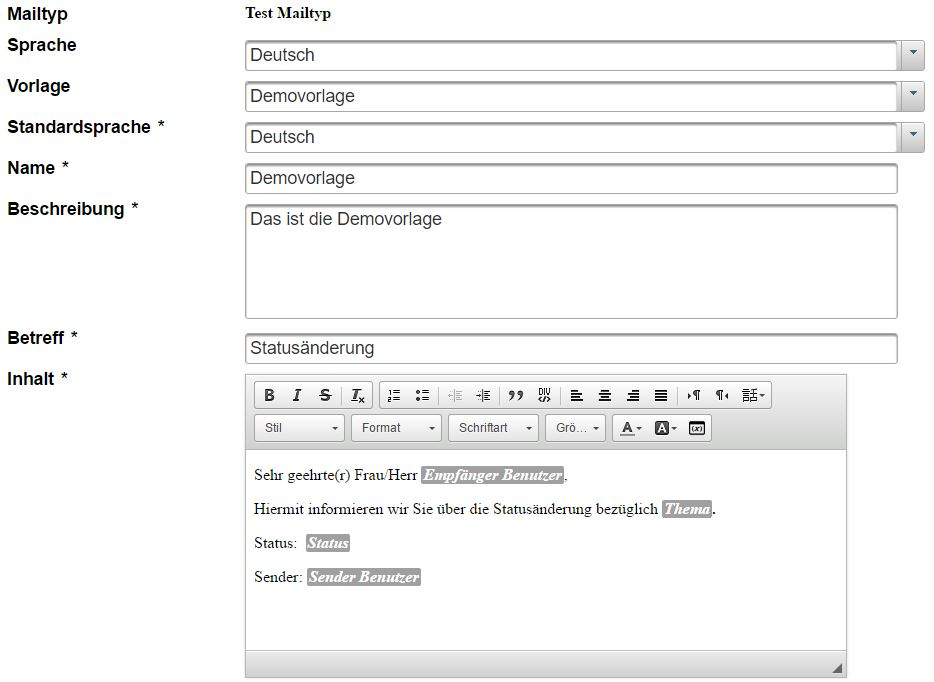
\includegraphics[scale=0.5]{demo_web_app_empty_view_part_1}
\caption{Das Formular für die Verwaltung der Vorlagen}
\label{fig:demo_web_app_empty_view_part_1}
\end{figure}
\ \newline
Die Abbildung \ref{fig:demo_web_app_empty_view_part_2} zeigt, den Teil der Webseite, der die relevanten Daten einer Vorlage anzeigt.

\begin{figure}[h]
\centering
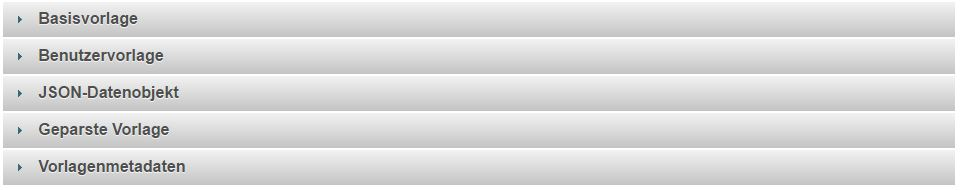
\includegraphics[scale=0.5]{demo_web_app_empty_view_part_2}
\caption{Die Anzeige der relevanten Daten einer Vorlage}
\label{fig:demo_web_app_empty_view_part_2}
\end{figure}
\ \newpage

\subsubsection{Basisvorlage}
Der Quelltext \ref{prog:demo_web_app_data_decorator} zeigt die \emph{Freemarker}-Basisvorlage, die von allen benutzerdefinierten Vorlagen ausgeprägt wird. Sie stellt das \emph{HTML}-Gerüst zur Verfügung, da die Benutzervorlagen nur den Inhalt innerhalb des \emph{HTML-Tags Body} bereitstellen.
\begin{program}[h]
\caption{Die \emph{Freemarker}-Basisvorlage}
\label{prog:demo_web_app_data_decorator}
\begin{HtmlCode}
<#macro includeMacro templateName>
    <#include "${templateName}" encoding="UTF-8">
</#macro>
<!DOCTYPE html>
<html lang="en">
<meta http-equiv="Content-Type" content="text/html; charset=utf-8">
<body>
<div style="margin: 10px;">
    <div style="padding: 5px;">
    <@includeMacro templateName="${TEMPLATE_NAME}" />
    </div>
    <div style="padding: 5px;">
    <@includeMacro templateName="${FOOTER_TEMPLATE}" />
    </div>
</div>
</body>
</html>
\end{HtmlCode}
\end{program}
%$ : otherwise everything afterwards is marked green
\ \newline
Die enthaltenen Variablen werden von der \emph{Template-Engine} \emph{Freemarker} durch die Vorlagen ersetzt:
\begin{itemize}
	\item\emph{TEMPLATE\_NAME} ist die Variable, die den Namen für die einzufügende Vorlage definiert.
	\item\emph{FOOTER\_TEMPLATE} ist die Variable, die den Namen für die einzufügende Vorlage für die Fußnote des \emph{HTML}-Dokuments definiert.
\end{itemize}

\subsubsection{Benutzervorlage}
Der Quelltext \ref{prog:demo_web_app_data_template} zeigt die \emph{Freemarker}-Vorlage, die von den BenutzerInnen erstellt wird. Die Vorlage enthält zwar \emph{HTML-Markup}, aber nur den Inhalt des \emph{HTML-Tags-Body}. Sie stellt daher kein vollständiges \emph{HTML}-Dokument dar, wofür gerade die Basisvorlage aus dem Quelltext \ref{prog:demo_web_app_data_decorator} implementiert wurde.
\newpage

\begin{program}[h]
\caption{Die \emph{Freemarker}-Vorlage der BenutzerIn}
\label{prog:demo_web_app_data_template}
\begin{HtmlCode}
<p>Sehr geehrte(r) Frau/Herr&nbsp;
${(cc.module.di["RECIPIENT_USER"])
!("variable: 'RECIPIENT_USER' not found")},</p>
<p>Hiermit informieren wir Sie &uuml;ber die Status&auml;nderung 
bez&uuml;glich&nbsp;<strong>
${(cc.module.di["TOPIC"])!("variable: 'TOPIC' not found")}.</strong></p>
<p>Status: &nbsp;
${(cc.module.di["STATUS"])!("variable: 'STATUS' not found")}</p>
<p>Sender:&nbsp;
${(cc.module.di["SENDER_USER"])!("variable: 'SENDER_USER' not found")}
</p>
<p>&nbsp;</p>
\end{HtmlCode}
\end{program}

\subsubsection{Serialisiertes \emph{JSON}-Datenobjekt}
Der Quelltext \ref{prog:demo_web_app_data_json} zeigt die serialisierte \emph{JSON}-Zeichenkette, die beim Erstellen einer \emph{E-Mail} generiert wird und in der Datenbank persistent gehalten wird. Mit diesen Daten kann eine \emph{E-Mail} auf Basis dieser Vorlage jederzeit wiederhergestellt werden.

\begin{program}[h]
\caption{Das \emph{JSON}-Datenobjekt}
\label{prog:demo_web_app_data_json}
\begin{JsCode}
{
  "@type" : "template-data-json",
  "template_metadata" : {
    "@type"         : "template-metadata-json",
    "id"            : 1,
    "version"       : 1,
    "locale"        : "de",
    "zoneId"        : "Europe/London",
    "variableCount" : 4
  },
  "data" : {
    "cc" : {
      "module" : {
        "di" : {
          "STATUS"         : "Inatkiv",
          "RECIPIENT_USER" : "Hugo Maier",
          "TOPIC"          : "BenutzerIn Status geändert",
          "SENDER_USER"    : "Thomas Herzog"
        }
      }
    }
  }
}
\end{JsCode}
\end{program}

\subsubsection{Ausgeprägte Benutzervorlage}
Der Quelltext \ref{prog:demo_web_app_data_parsed_template} zeigt die ausgeprägte Benutzervorlage. Die Variablen der Vorlage aus dem Quelltext  \ref{prog:demo_web_app_data_template} wurden durch die serialisierten Werte des \emph{JSON}-Datenobjekts aus dem Quelltext \ref{prog:demo_web_app_data_json} ersetzt.

\begin{program}[h]
\caption{Die ausgeprägte Benutzervorlage}
\label{prog:demo_web_app_data_parsed_template}
\begin{HtmlCode}
<!DOCTYPE html>
<html lang="en">
    <meta http-equiv="Content-Type" content="text/html; charset=utf-8">
<body>
<div style="margin: 10px;">
    <div style="padding: 5px;">
        <p>Sehr geehrte(r) Frau/Herr&nbsp;Hugo Maier,</p>

        <p>
            Hiermit informieren wir Sie &uuml;ber die 
            Status&auml;nderung bez&uuml;glich&nbsp;
            <strong>BenutzerIn Status geändert.</strong>
        </p>

        <p>Status: &nbsp;Inatkiv</p>

        <p>Sender:&nbsp;Thomas Herzog</p>

        <p>&nbsp;</p>
    </div>
    <div style="padding: 5px;">
    </div>
</div>
</body>
</html>
\end{HtmlCode}
\end{program}

\subsubsection{Vorlagenmetadaten}
Der folgende Text zeigt die Zeichenketten, welche die in Abschnitt \ref{sec:abstractTemplateMetadata} vorgestellte Klasse \emph{AbstractTemplateMetadata} produziert. Diese Ausgabe ist nur für Entwicklungszwecke interessant und zeigt die aktuellen Metadaten der Vorlage aus dem Quelltext  \ref{prog:demo_web_app_data_template}.

\begingroup
    \fontsize{9pt}{11pt}\selectfont
    \begin{verbatim}  
===============================================================
FreemarkerTemplateMetadata
===============================================================
id                  : 1
version             : 1
length              : 482
variables (valid)   : 4
contract  : com.clevercure.mailing.demo.logic.variable.TemplateVariable
id        : cc.module.di.SENDER_USER
name      : SENDER_USER
label-key : SENDER_USER
info-key  : SENDER_USER


contract  : com.clevercure.mailing.demo.logic.variable.TemplateVariable
id        : cc.module.di.STATUS
name      : STATUS
label-key : STATUS
info-key  : STATUS


contract  : com.clevercure.mailing.demo.logic.variable.TemplateVariable
id        : cc.module.di.RECIPIENT_USER
name      : RECIPIENT_USER
label-key : RECIPIENT_USER
info-key  : RECIPIENT_USER


contract  : com.clevercure.mailing.demo.logic.variable.TemplateVariable
id        : cc.module.di.TOPIC
name      : TOPIC
label-key : TOPIC
info-key  : TOPIC

variables (invalid) : 0
    \end{verbatim}  
\endgroup

\subsection{Verwendung in einer Geschäftslogik}
Der Quelltext \ref{prog:emailService} zeigt die Schnittstelle \emph{EmailService}, die spezifiziert, wie über eine Geschäftslogik \emph{E-Mails} erstellt werden können. Folgende Auflistung erklärt die definierten Methoden der Schnittstelle \emph{EmailService}:
\begin{itemize}
	\item\emph{create(EmailDTO dto)} erstellt eine \emph{E-Mail}.
	\item\emph{create(List<EmailDTO> dtos)} erstellt mehrere \emph{E-Mails}.
	\item\emph{createAfterSuccess(EmailDTO dto)} erstellt eine \emph{E-Mail}, nach dem erfolgreichem Beenden einer Transaktion.
	\item\emph{createAfterSuccess(List<EmailDTO> dto)} erstellt mehrere \emph{E-Mails}, nach dem erfolgreichem Beenden einer Transaktion.
\end{itemize} 
\ \newpage

\begin{program}
\caption{Die Schnittstelle \emph{EmailService}}
\label{prog:emailService}
\begin{JavaCode}
public interface EmailService extends Serializable {

    void create(EmailDTO dto);

    void create(List<EmailDTO> dtos);

    void createAfterSuccess(EmailDTO dto);

    void createAfterSuccess(List<EmailDTO> dtos);
    
}
\end{JavaCode}
\end{program}
\ \newline
Der Quelltext \ref{prog:emailServiceCdiEventImpl} zeigt die Klasse \emph{EmailServiceCdiEventImpl}, welche die Schnittstelle \emph{EmailService} implementiert und die \emph{E-Mails} über \emph{CDI-Events} erstellt. 
\newline
\newline
Objekte der Klasse \emph{CreateEmailsEvent} sind \emph{Event}-Objekte, die alle benötigten Daten für die Erstellung einer \emph{E-Mail} halten und nach dem Auslösen eines \emph{Events} über den \emph{CDI-Event-Bus} verarbeitet werden. 
\newline
\newline
Es werden Objekte des Datentyps \emph{javax.enterprise.Event} injiziert, welche mit dem Datentyp \emph{CreateEmailsEvent} typisiert sind. Die Injektionspunkte der \emph{Events} wurden mit den im Folgenden aufgelisteten Annotationen qualifiziert:
\begin{itemize}
	\item\emph{@Immediate} ist die Annotation, die das injizierte \emph{Event} für die sofortige Ausführung qualifiziert.
	\item\emph{@AfterSuccess} ist die Annotation, die das injizierte \emph{Event} für die Ausführung nach dem erfolgreichen Abschluss einer Transaktion qualifiziert.
\end{itemize}
\ \newline
Durch die Qualifizierung der \emph{Event}-Injektionspunkte wird erreicht, dass verschiedene Beobachtermethoden implementiert werden können, welche die ausgelösten Events in unterschiedlichen Phasen der Transaktion behandeln.
\newpage

\ \begin{program}
\caption{Die Klasse \emph{EmailServiceCdiEventImpl}}
\label{prog:emailServiceCdiEventImpl}
\begin{JavaCode}
@RequestScoped
@Transactional(Transactional.TxType.SUPPORTS)
public class EmailServiceCdiEventImpl implements EmailService {

    @Inject
    @Immediate
    private Event<CreateEmailsEvent> createImmediateEvent;
    
    @Inject
    @AfterSuccess
    private Event<CreateEmailsEvent> createAfterSuccessEvent;

    @Override
    @Transactional(Transactional.TxType.REQUIRED)
    public void create(EmailDTO dto) {
        createImmediateEvent.fire(new CreateEmailsEvent(dto));
    }

    @Override
    @Transactional(Transactional.TxType.REQUIRED)
    public void create(List<EmailDTO> dtos) {
        createImmediateEvent.fire(new CreateEmailsEvent(dtos));
    }

    @Override
    public void createAfterSuccess(EmailDTO dto) {
        createAfterSuccessEvent.fire(new CreateEmailsEvent(dto));
    }

    @Override
    public void createAfterSuccess(List<EmailDTO> dtos) {
        createAfterSuccessEvent.fire(new CreateEmailsEvent(dtos));
    }
    
}
\end{JavaCode}
\end{program}
\ \newline
Der Quelltext \ref{prog:businessServiceImpl} zeigt die Klasse \emph{BusinessServiceImpl}, welche die Geschäftslogik simuliert, die über die Schnittstelle \emph{EmailService} \emph{E-Mails} erstellt. Die zu erstellende \emph{E-Mail} wird durch ein Objekt der Klasse \emph{EmailDTO} repräsentiert, das alle benötigten Informationen für das Erstellen einer \emph{E-Mail} enthält. Das Objekt des Datentyps \emph{EmailService} wird über Injektion von der \emph{CDI}-Umgebung bereitgestellt. Wie im Kapitel \ref{cha:Zielsetzung} vorgegeben, dürfen die Anwendungen nicht wissen, wie \emph{E-Mails} erstellt werden, was über die Schnittstelle \emph{EmailService} realisiert wurde. Einer Geschäftslogik ist die konkrete Implementierung der Schnittstelle \emph{EmailService} nicht bekannt und daher auch nicht, dass die \emph{E-Mails} über \emph{CDI-Events} bzw. deren Beobachtermethoden erstellt werden.
\newline
\newline
Die \emph{E-Mails} werden innerhalb der von der Klasse \emph{BusinessServiceImpl} geöffneten Transaktion erstellt. Es ist nicht möglich eine Transaktion in einer Beobachtermethode zu öffnen, da die \emph{Events} immer in der Komplettierungsphase der geöffneten Transaktion behandelt werden und es keine Möglichkeit gibt, dies zu umgehen.
\begin{program}[h]
\caption{Die Klasse \emph{BusinessServiceImpl}}
\label{prog:businessServiceImpl}
\begin{JavaCode}
@RequestScoped
@Transactional(Transactional.TxType.REQUIRED)
public class BusinessServiceImpl implements BusinesService {

    @Inject
    private EmailService emailService;
    
    @Override
    public void doBusinessEmailImmediate() {
        emailService.create(createEmailDto());
    }

    @Override
    public void doBusinessEmailAfterSuccess() {
        emailService.createAfterSuccess(createEmailDto());
    }

    private EmailDTO createEmailDto() {
        final String email = "herzog.thomas8@gmail.com";
        final Long mailUserId = 1L;
        final List<Long> mailTypeIds = Collections.singletonList(1L);
        final Locale locale = Locale.US;
        final ZoneId zone = ZoneId.systemDefault();
        final Map<Object, Object> userData = 
        	new HashMap<Object, Object>() {{
                put(TemplateVariable.SENDER_USER, "Thomas Herzog");
                put(TemplateVariable.RECIPIENT_USER, "Hugo Maier");
                put(TemplateVariable.TOPIC, "User status changed");
                put(TemplateVariable.STATUS, "Inactive");
            }};            
        return new EmailDTO(email, 
        					locale, 
        					zone, 
        					mailUserId, 
        					userData, 
        					mailTypeIds);
    }
    
}
\end{JavaCode}
\end{program}
\ \newline
Folgende Auflistung erklärt die Attribute, die beim Erstellen eines Objekts der Klasse \emph{EmailDTO} angegeben werden müssen:
\begin{itemize}
	\item\emph{email} ist die Zeichenkette, welche die \emph{E-Mail}-Adresse definiert.
	\item\emph{mailUserId} ist der Bezeichner der internen \emph{Mail}-BenutzerIn, welcher die \emph{E-Mail} in der Datenbank erstellt.
	\item\emph{mailTypeIds} ist die Menge der Bezeichner, welche die \emph{Mail}-Typen repräsentieren. Jedem \emph{Mail}-Typ ist eine Voralge zugeordnet.
	\item\emph{locale} ist das Objekt der Klasse \emph{java.util.Locale}, das die Sprache definiert.
	\item\emph{zone} ist das Objekt der Klasse \emph{java.time.ZoneId}, das die Zone für die Datums- und Zeitformatierung definiert.
	\item\emph{userData} ist der assoziative Behälter, der die Benutzerdaten enthält, die bei der Ermittlung der aktuellen Werte der Variablen verwendet werden können.
\end{itemize}
\ \newline
In diesem Kapitel wurde die Implementierung der Spezifikation, die in Kapitel \ref{cha:Lösungskonzept} vorgestellt wurde, behandelt. Das nächste Kapitel \ref{cha:Analyse} beschäftigt sich mit den Tests und der Analyse der in diesem Kapitel behandelten Implementierungen.